% !TeX encoding = UTF-8
% !TeX spellcheck = pt_BR
% !TeX root = ../template.tex
% !Tex tags =

\question[10]

Traduza cada uma das sentenças abaixo em lógica de predicados usando: $Triangulo(x)$, $Circulo(X)$, $Quadrado(X)$, $Branco(X)$, $Cinza(X)$, $Preto(X)$, $Grande(X)$, $Pequeno(X)$. Depois disso, diga se cada sentença é verdadeira ou falsa usando uma instância do Tarski World apresentado na figura abaixo.

\begin{figure}[h!]
	\centering
	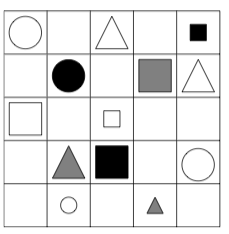
\includegraphics[width=0.3\linewidth]{10-logica-de-predicados-semantica/images/tarski-world}
\end{figure}


\begin{parts}
	\part \tf[V] \textit{``Não existe triângulos pretos''} \newline \fillin[$\neg \exists x (Triangulo(x) \wedge Preto(x)) $][14cm]
	\part \tf[V] \textit{``Todos os triângulos brancos são grandes''} \newline \fillin[$\forall x ((Triangulo(x)  \wedge Branco(x)) \rightarrow Grande(x)) $][14cm]
	\part \tf[F] \textit{``Todos os triângulos grandes são brancos''} \newline \fillin[$\forall x ((Triangulo(x)  \wedge Grande(x)) \rightarrow Branco(x)) $][14cm]
	\part \tf[F] \textit{``Todos quadrados são pretos e grandes''} \newline \fillin[$\forall x (Quadrado(x) \rightarrow (Preto(x)  \wedge Grande(x))) $][14cm]
\end{parts}
	